\subsection{Kleinste gemeinsame Vielfache (kgv)}

\hfill \break
Das kgv wird errechnet in dem man jeden Faktor in der jeweils höchst vorkommenden Potenz miteinenader multipliziert.\\

\hfill \break
Das kgv wird wie folged berechnet:\\
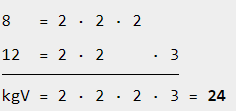
\includegraphics[scale=0.8]{KGV}

\hfill \break
Example: Ermittling des kgv von 24 und 30\\
\fboxrule=0.8pt \fcolorbox{lightgray}{lightgray}{%
    \begin{tabular}{c|c||c|c}
        24 & 2 & 30 & 2 \\
        12 & 2 & 15 & 2 \\
        6  & 2 & 5  & 5 \\
        3  & 3 & 4  &   \\
        1  &   &    &   \\
    \end{tabular}}
$kgv(24,30) = 2^3*3^1*5^1 =120$